\documentclass[twocolumn,9pt]{jsproceedings}
\RequirePackage[l2tabu,orthodox]{nag}  % 古いコマンドやパッケージを使用した場合に警告する
%\usepackage{subcaption}
\usepackage[all,warning]{onlyamsmath}  % amsmath が提供しない数式環境を使用した場合に警告する
% \usepackage{flushend}  % 最終ページの2カラムの左右の高さを揃える
\usepackage{here} %図の場所の指定で[h](ここに貼る)を指定するためのパッケージ
\usepackage[dvipdfmx]{graphicx} %dvipdfmxはjpgやpngの張り込みのために使用
%\usepackage{graphicx}

% タイトル
\title{新卒だけどつくばチャレンジ出るよチームの\\つくばチャレンジ2024での取り組み}

\author{○池邉 龍宏\authorrefmark{1}、海老田 そら\authorrefmark{1}、春山 健太\authorrefmark{1}、大澤 来実\authorrefmark{1}\\森下 敢太\authorrefmark{1}、
深谷 和俊\authorrefmark{1}、藤江 謙伸\authorrefmark{1}、新宮 義規\authorrefmark{1}}

\etitle{Our Team's Efforts in Tsukuba Challenge 2024 as a New Graduate Participant}

\eauthor{○Tatsuhiro IKEBE\eauthorrefmark{1}、Sora Ebita\eauthorrefmark{1}、Kenta Haruyama\eauthorrefmark{1}、Kurumi Osawa\eauthorrefmark{1}\\Kanta Morisita\authorrefmark{1}
Fukaya Kazuya\eauthorrefmark{1}、Fujie Kenshin\eauthorrefmark{1}、Shingu Yoshiki\eauthorrefmark{1}}

\affiliation{新卒だけどつくばチャレンジ出るよ}

\begin{document}
\maketitle

\authorreftext{1}{社会人}
\eauthorreftext{1}{Department of Advanced Robotics、Faculty of Advanced Engineering、Chiba Institute of Technology}

% 本文
\section{緒言}

新卒だけどつくばチャレンジ出るよチームは同じ会社内にて
つくばチャレンジに参加したいという
意志のあるメンバーが集まったチームである。
チームメンバーは2024年に新規学卒者(新卒)の計8名のメンバー構成で作成された。
過去につくばチャレンジに参加したことがある方や初めて参加する方がそれぞれ在籍している。

本チームの目的は、
新卒においても、つくばチャレンジに参加することが可能であることを証明することである。
また、本チームの活動を元に、来年のつくばチャレンジで新卒として参加するチームが増えるようにしていきたいと考えている。
この目的を達成するために各目標を
\begin{itemize}
  \item[1] 参加登録
  \item[2] 作成した機体の車検を通す
  \item[3] 機体から得られたセンサ情報できれいな地図を取得
  \item[4] 確認走行区間を完走
\end{itemize}
とした。


本稿では、目標に対する取り組みと結果について説明する。
本稿の構成は次の通りである。
2章ではロボットのソフトウェア、ハードウェア構成について説明し、
3章では本走行の結果と見つかった課題を示す。
4章では本年度のつくばチャレンジで利用しなかった研究室での取り組みを紹介し、
5章では結言を述べる。

\section{ロボットの構成}

\subsection{ハードウェア構成}
ロボットの外観を図\ref{fig:robot}に示す。
本ロボットは、ODrive社製の既製品である、BotWheel Explorer Kit\cite{RTshop}がベースになっている。

\begin{figure}[h]
  \begin{center}
    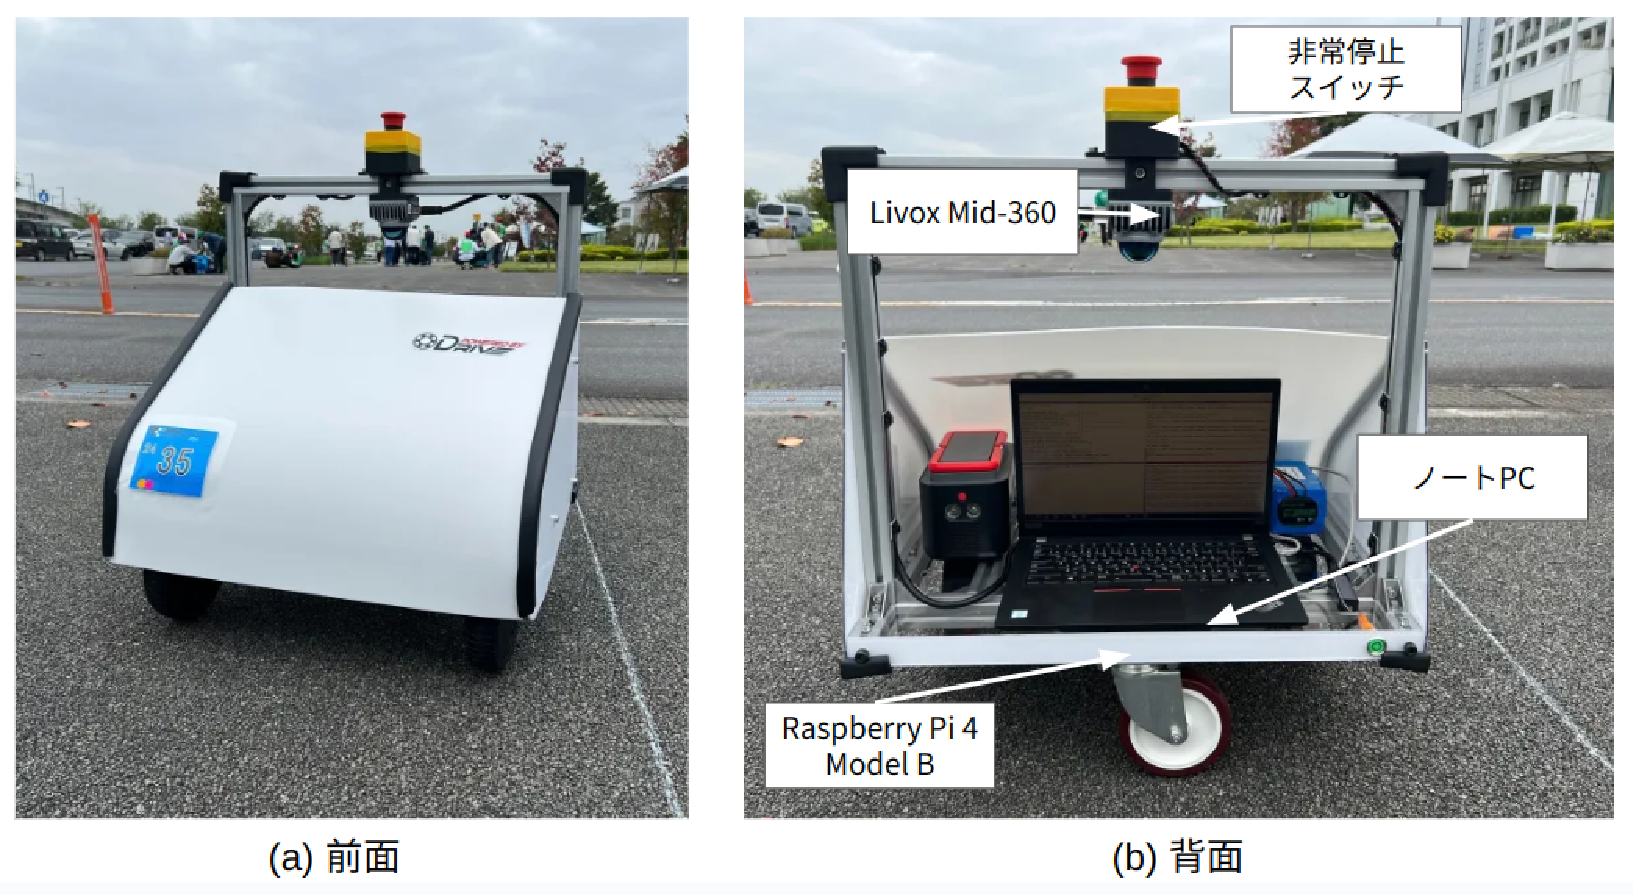
\includegraphics[width=1.0\linewidth]{figs/0_robot.pdf}
    \caption{チームの機体}
    \label{fig:robot}
  \end{center}
\end{figure}

\begin{figure}[h]
  \begin{center}
    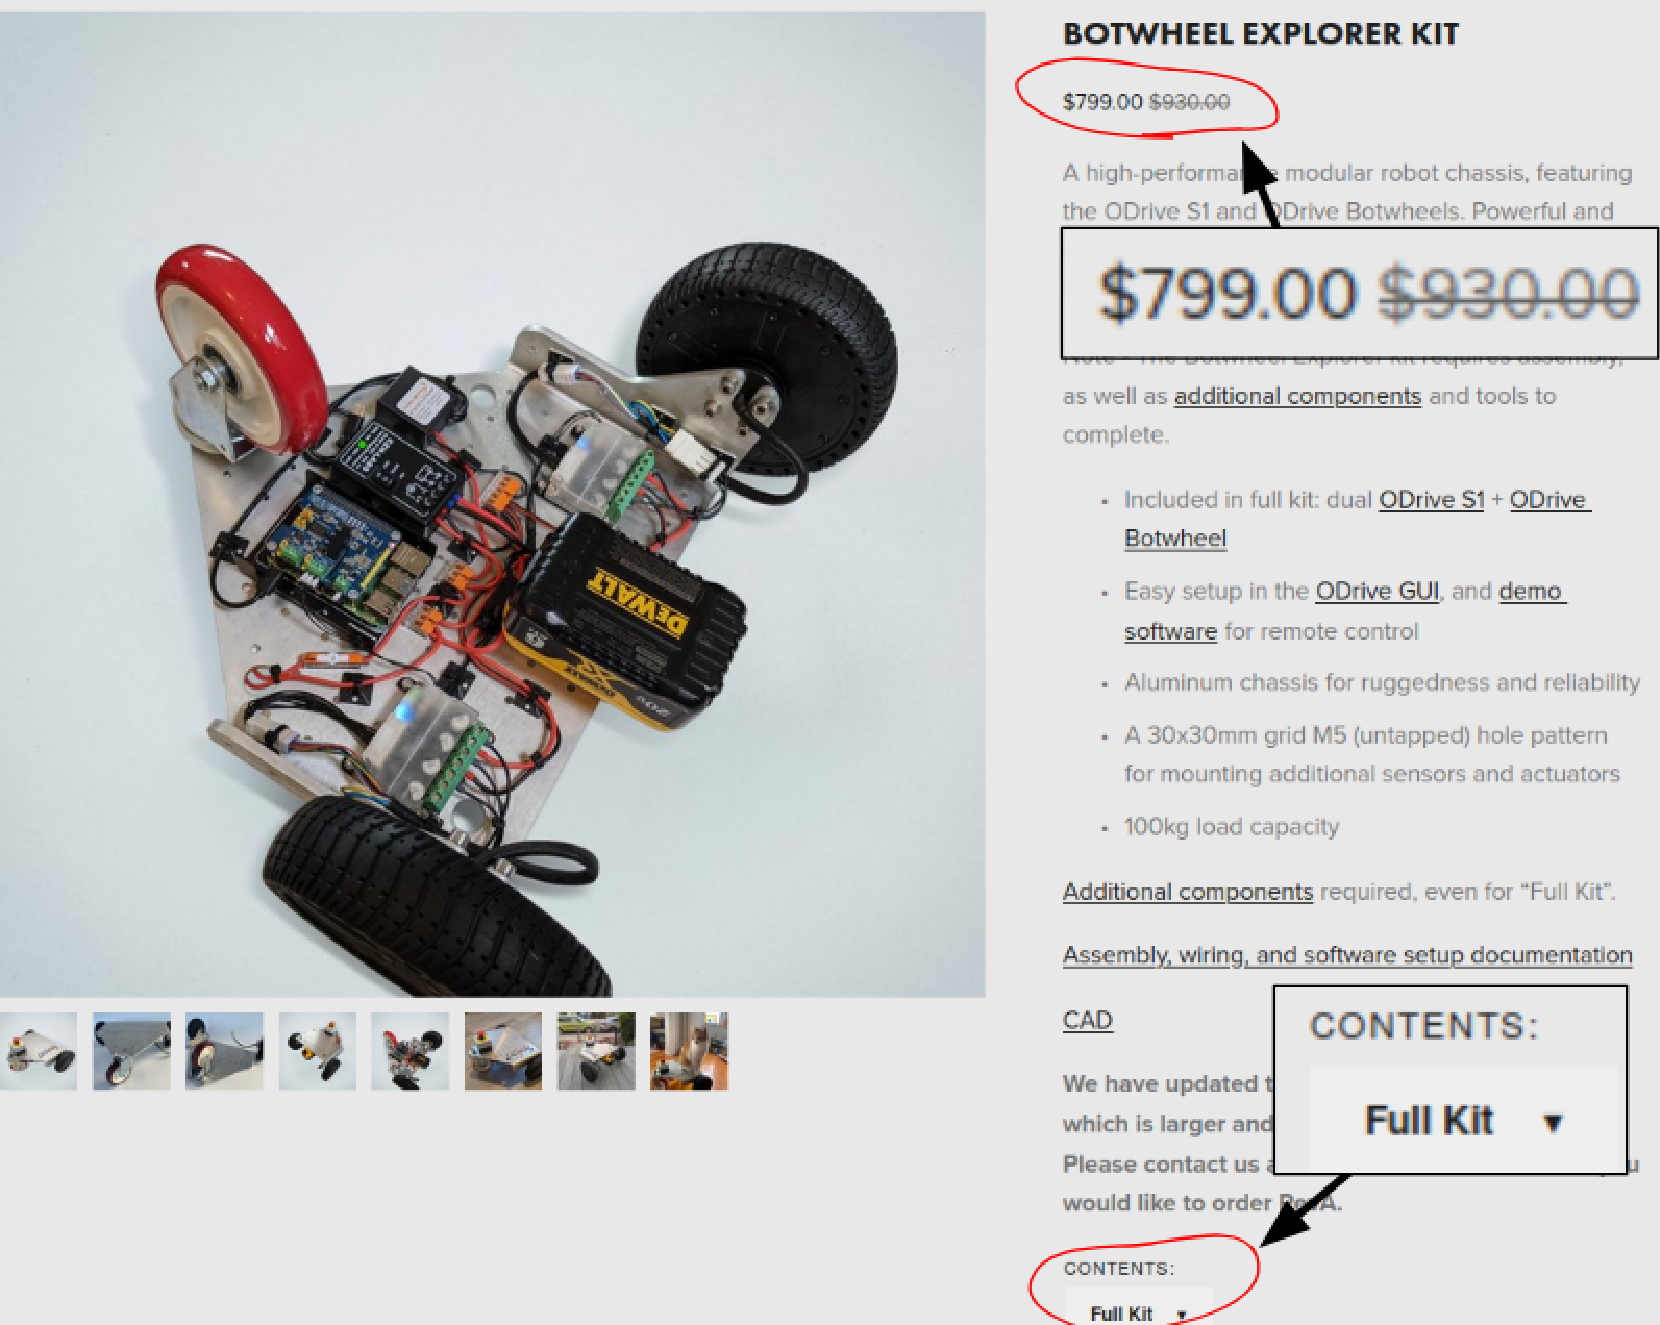
\includegraphics[width=0.8\linewidth]{figs/b_kit_price.pdf}
    \caption{BotWheel Explorer Kitの金額および内容について}
    \label{fig:b_robot_price}
  \end{center}
\end{figure}

このロボットをベースに使用する理由はなんといっても安さである。図\ref{fig:b_robot_price}のように、驚くべきことに\$799で購入することが可能である。
さらに、購入内容としては「Full Kit」という魅力的な内容である。
これは他のロボットの購入サイトを比較しても、類を見ないものであるため、ありがたく購入をさせていただいた。
しかし、「Full Kit」といっても、図\ref{fig:b_robot_price}のような電装部品も込みというわけではなかった。
商品ページの画像にはいかにも全て揃っているように間違える可能性があるので注意する必要がある。
また、購入のタイミングでは円相場と海外手数料について考慮する必要がある。

Full Kitを購入した場合に梱包されているものを表に示す。
内容としては、駆動用のインホイールモータ、制御用のモータドライバ、
モータの取り付けおよび機体のボーディのためのシャーシ、モータドライバとインホイールモーター間の通信に必要な
CANハーネスが梱包等が梱包されている。
\begin{table}[h]
  \centering
  \begin{tabular}{|l|c|l|}
      \hline
      \multicolumn{3}{|c|}{\textbf{BotWheel Explorer Kit(Full Kit)}} \\
      \hline
      部品 & 数量 & 詳細 \\
      \hline
      ODrive S1 & 2 & モータドライバー \\
      ODrive Botwheel & 2 & インホイールモーター(エンコーダ付き) \\
      Chassis Plate & 1 & シャーシ \\
      Caster & 1 & キャスター \\
      CAN harnesses & 2 & CAN ハーネス \\
      \hline
  \end{tabular}
  \caption{BotWheel Explorer Kit の部品一覧}
  \label{tab:botwheel_kit}
\end{table}


BotWheel Explorer Kitは、前方の2つの駆動輪と後方の1つの受動輪が、三角形の金属板に取り付けられている足回りだけのユニットであり、全面の保護カバーはない。
そこで、図\ref{fig:robot_flame}(a)のように20×20mmのアルミフレームを金属板に固定し、(b)に示すように〇〇のカバーを取り付けることで雨除けとした。
〇〇は、厚さ3mmで、手で簡単に曲げられることから湾曲した形状を作りやすいため採用した。
さらに、金属板にはナットが飛び出ている箇所があるなど平らなスペースが小さいことから、アルミフレームの上に四角形の〇〇板を取り付け、ノートPCやバッテリーを搭載できるスペースを広げた。
また、ロボットの最低高さ600mmという寸法制限と運搬のしやすさを考え、アルミフレームを上部に伸ばし台車の持ち手のような構造とした。
非常停止スイッチ・3次元LiDARは、3Dプリンタで治具を製作しアルミフレームに固定した。
%また、手動操作用のコントローラー置き場・信号検出用のスマートフォン置き場も、3Dプリンタで製作しアルミフレームに取り付けた。\par

アルミフレームや治具等の設計には、Fusion360\cite{Fusion360}を使用した。
ただ、無料ライセンスではチーム開発ができなかったため、制作したCADモデルを共有する際にはOnshape\cite{Onshape}を使用した。



計算機については、ノートPCを各ロボットに搭載して使用した。
昨年は、1チームが計算機としてRaspberry Pi 4 Model Bのみを
使用して自律走行を実現した\cite{池邉2022}。
しかし本年度については、
Raspberry Pi上でROS 2を実行するための
技術的な課題が解決しておらず、
ノートPCを使用することとなった。
この場合、Raspberry Pi Catには、
ノートPCと制御用のRaspberry Piの2台の計算機が搭載されることとなる。
センサ構成としては、各チームの機体に外界センサとして
2次元LiDAR、3次元LiDAR、内界センサとしてIMUを搭載した。

\begin{figure}[h]
  \begin{center}
    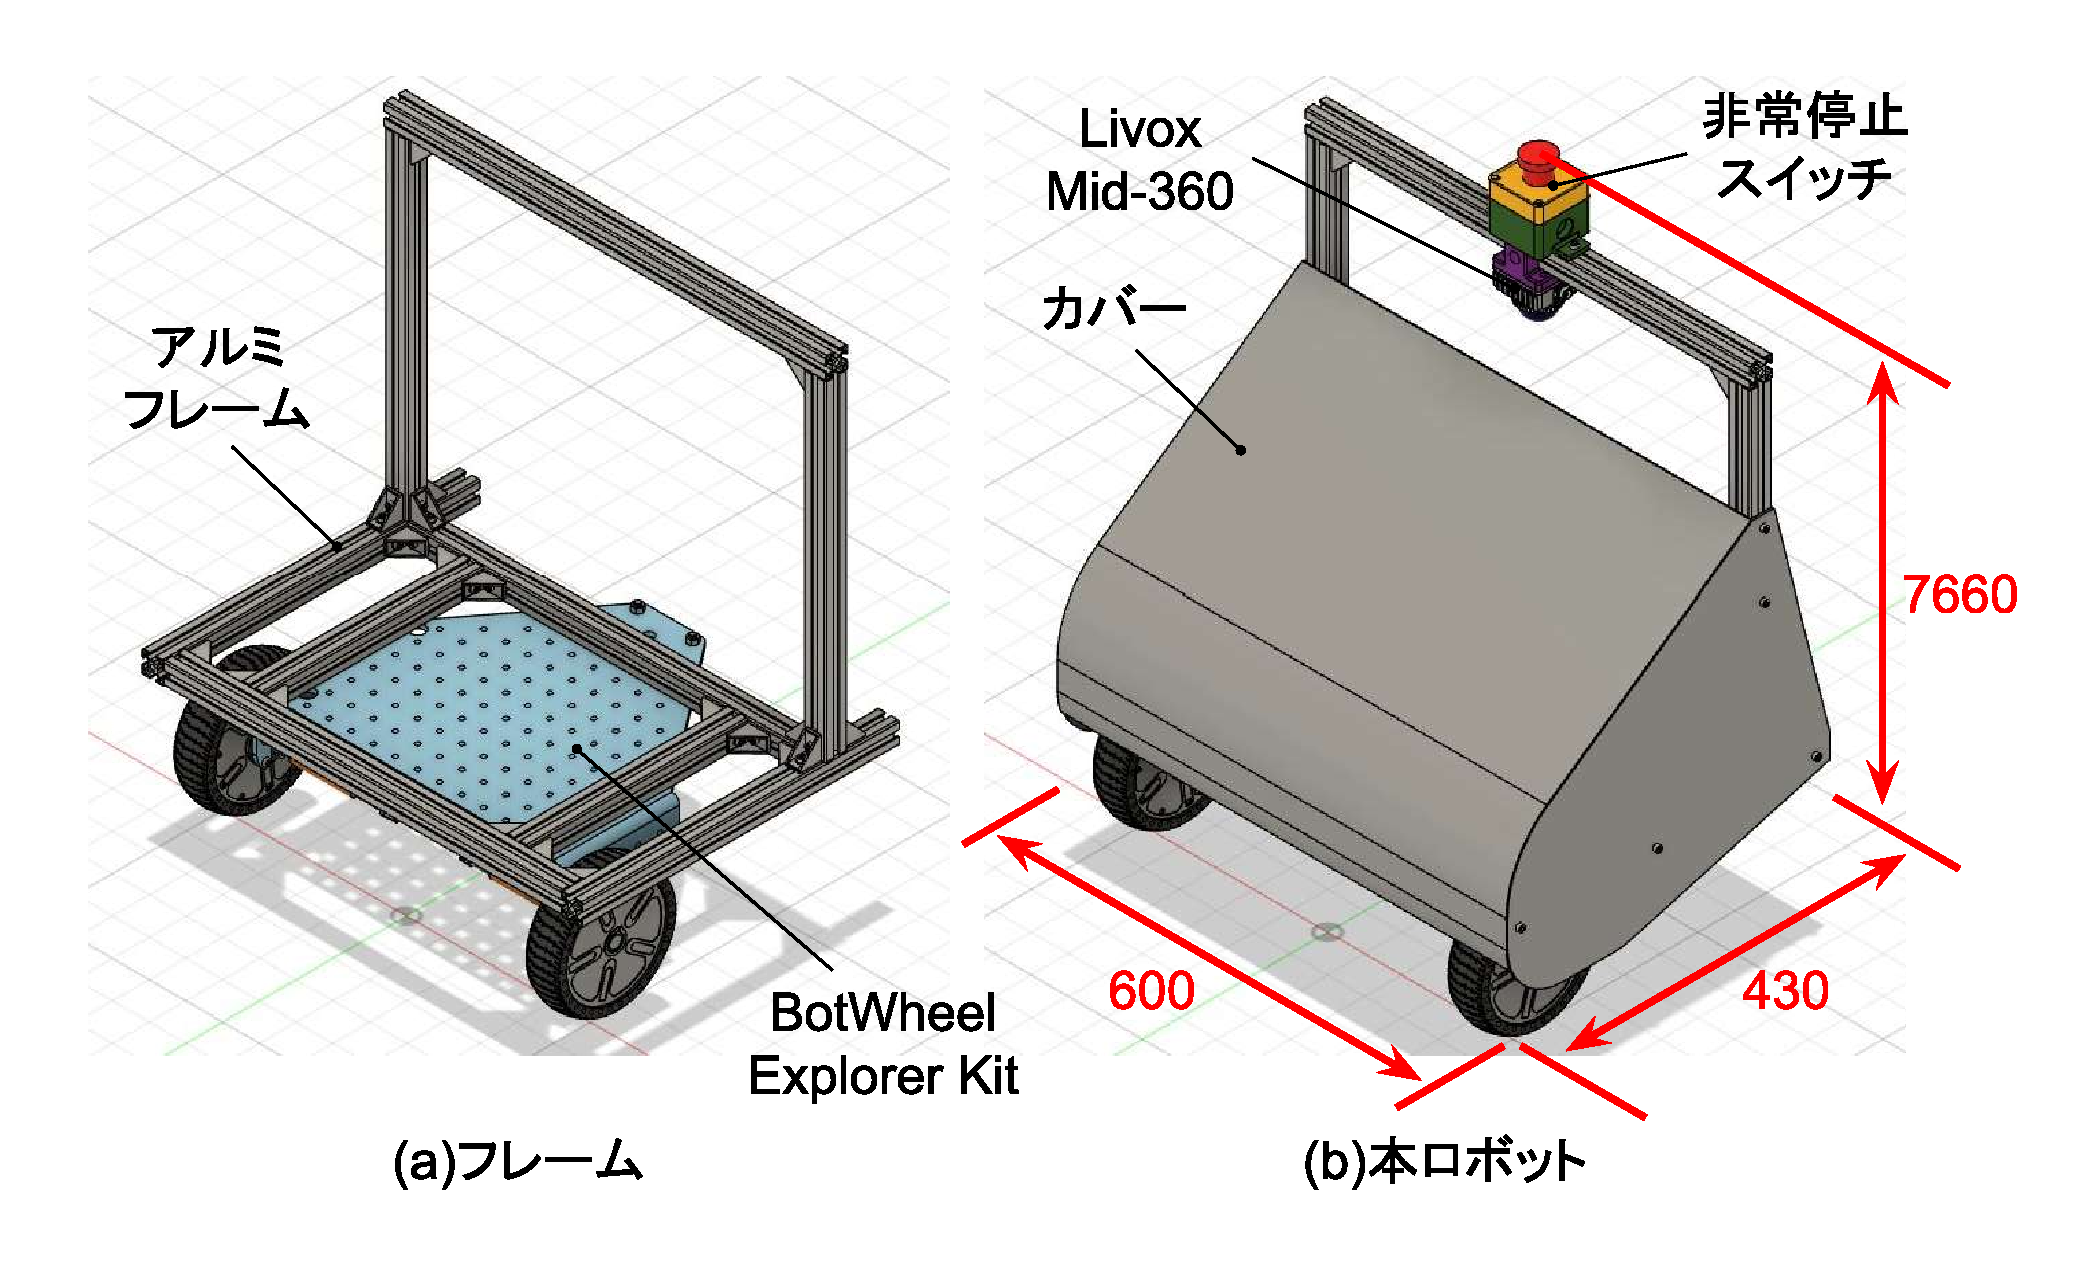
\includegraphics[width=1.0\linewidth]{figs/robot_flame.pdf}
    \caption{メカ設計}
    \label{fig:robot_flame}
  \end{center}
\end{figure}

\subsection{ソフトウェア構成}

ソフトウェアについては、
本年度は、3チーム全てがROS 2をベースに構築した。
昨年度まではROS\cite{ROS}を使用していたが、
ROSの最終リリースであるROS Noetic Ninjemysが2025年5月に
サポート終了を迎えることを受けてのことである。

他、各チームの特徴について、
次節以降で説明する。


\subsection{ツナチーム}


\subsubsection{概要}
ツナチームは、ROS 2をベースに自作ナビゲーションスタックを作成して使用した。
%図\ref{fig:robot}の小型移動ロボット上で動作させ、
%をさせることを目的とした。
この自作ナビゲーションスタックは、
GitHub上のリポジトリuhobeike/ike\_nav\cite{ike_nav}
に公開している。
また、リポジトリの内容については
%「自作ナビゲーションスタックでつくばチャレンジ2023に挑戦してみた話」
\cite{ike_nav_detail}にまとめた。
%↑いちおう教育的観点で言うと、「記事内に金出した研究室とかその他関係者に謝辞入れやがれ自分のことしか書いてなくてよくないよこれ。」
%(言うの恥ずかしいので言わせないでほしい・・・)

このパッケージは「Nav2のような複雑な
システムではなく、シンプルで修正しやすいパッケージを作成したい」
という動機で作成した。
ソフトウェアを再利用してフィードバックすることも重要であるが、
ブラックボックスのない
ソフトウェアパッケージを開発する方針も考えられたため、
開発に踏み切った。

%例えば、つくばチャレンジ中に何か解決したい問題が発生し、
%ソフトウェア上で解決したいとなった場合に、
%パラメータやコードに対して手を入れやすいメリットがあると考えている。

%uhobeike/ike\_navの作成に関する詳細については、

%↓いらない
%\subsubsection{使用したハードウェア}
%ツナチームでは、図\ref{fig:robot}の機体を自律走行させた。
%機体には、2つのコンピュータが搭載されている。
%一つ目は、計算用として、ノートPCを搭載した。
%このノートPC上でike\_navを動作させた。
%二つ目は、機体の制御用として、Raspberry Pi 4B+を搭載した。
%
%観測用のセンサは、2次元LiDARであるUST-30LX\cite{UST-30LX}を搭載した。
%このLiDARの捜査角度は、270[deg]であり、最大検出距離は60[m]である。


\subsubsection{ike\_navのシステム構成}

図\ref{fig:tuna_system}に、ike\_navのシステム構成を示す。
ike\_navは、地図、2次元LiDARからの観測情報(スキャン)、
ロボットのオドメトリを入力して受け入れ、
ある目標地点まで到達するための速度および推定した自己位置を出力する。

\begin{figure}[h]
  \begin{center}
    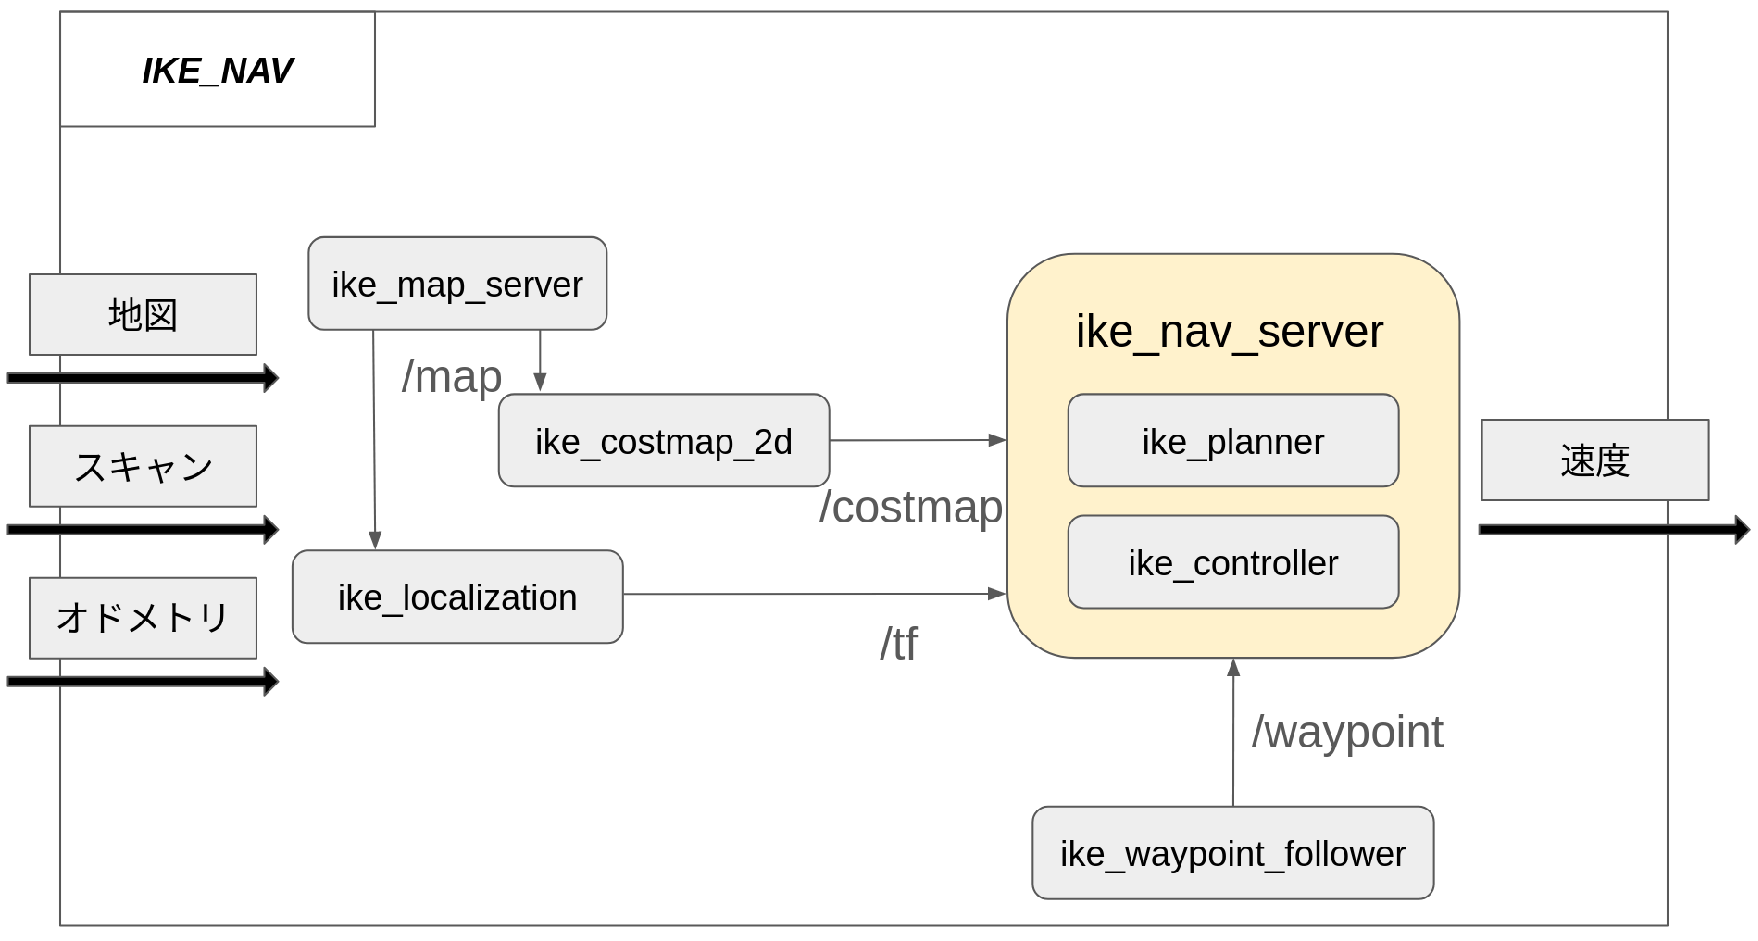
\includegraphics[width=1.0\linewidth]{figs/ike_nav.pdf}
    \caption{ツナチームのシステム構成}
    \label{fig:tuna_system}
  \end{center}
\end{figure}

ike\_navはメタパッケージであり、
自己位置推定、経路計画、経路追従などがそれぞれ別々にパッケージ化されている。
含まれるパッケージを列挙すると、次のようになる。
\begin{description}
  \item[・ike\_controller(経路追従):]経路、推定位置を入力し、速度を出力
  \item[・ike\_costmap\_2d(コストマップの管理):]地図、観測情報を入力し、コストマップを出力
  \item[・ike\_localization(自己位置推定):]観測情報、地図、ロボットのオドメトリを入力し、自己位置を出力
  \item[・ike\_map\_server(地図の管理):]pgmなどのデータからROS 2の占有格子地図を出力
  \item[・ike\_nav\_server(目標地点までの管理):]目標地点を入力し、到達するまでを管理
  \item[・ike\_planner(経路計画):]コストマップ、推定位置を入力し、経路を出力
  \item[・ike\_waypoint\_follower(複数目標地点の管理):]事前に設定した目標地点を辿るように管理
\end{description}

ike\_localization(自己位置推定)とike\_planner(経路計画)は、
それぞれつくばチャレンジでもよく用いられる
MCL(Monte Carlo Localization)\cite{fox1999etal}
とA*探索\cite{hart1968}を利用して実装した。
%最短経路を導出するアルゴリズムであり、
%他の最短経路法であるダイクストラ\cite{dijkstra1959}よりも
%速く最短経路を導出することができるため採用した。
ike\_planner(経路計画)のA*では、センサで観測した障害物
を回避する経路を導出するように実装した。
ike\_controller(経路追従)では、経路追従の手法として、
モデル予測制御(Model Predictive Control、MPC)\cite{alberto2006}を実装した。
MPCは、他の追従手法と比較して、計算コストが高いというデメリットがあるが、
経路に対する追従性が高いというメリットがあるため採用した。


\subsection{たまチーム}\label{sub:localization}
\subsubsection{概要}
たまチームは、ROS 2に移行されたemcl2パッケージ
emcl2\_ros2を用いて、
屋外でロボットに自律走行させた。
目標に関しては、つくばチャレンジ初参加のチームメンバーであることも考え、
無理に完走を目指さず、交差点手前までのナビゲーションということにした。

\subsubsection{使用したハードウェアとソフトウェア}

たまチームのシステムの構成を図\ref{fig:tama_system_diagram}に示す.
ロボットに搭載された2D LiDARとIMUから、
Raspberry Pi 4B+を介し、センサ情報をノートPCに送信する。
ノートPCでは自己位置推定、経路計画が行われ、
その結果として得られた制御指令がRaspberry Pi 4に返される。
マッピングにはslam\_toolboxを利用し、
経路計画にはNav2を利用した。
%また、自己位置推定においては、
%昨年度まで利用されていたemcl2パッケージを
%ROS 2に移行した、emcl2\_ros2利用している。

\begin{figure}[h]
  \begin{center}
    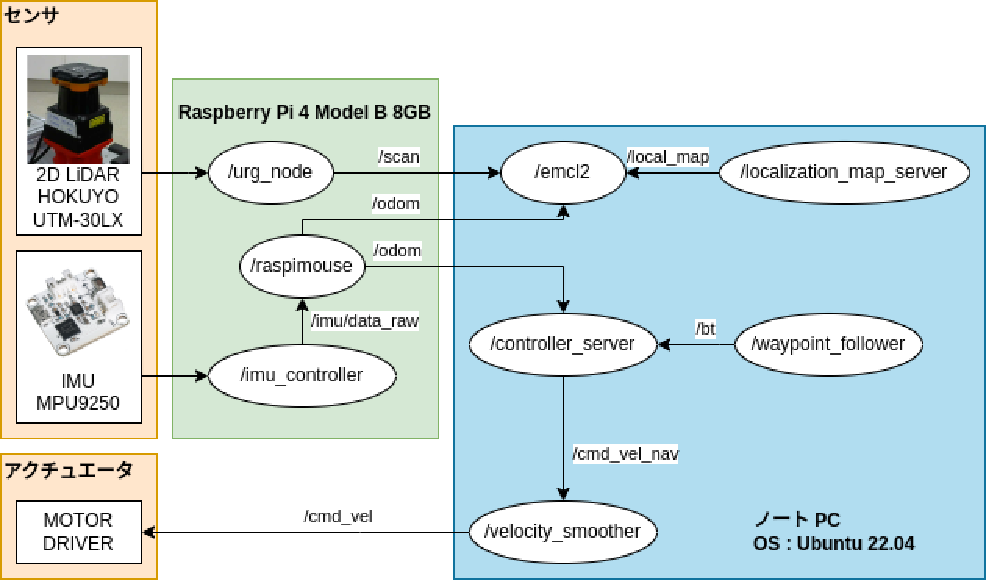
\includegraphics[width=1.0\linewidth]{figs/tama_system_diagram.pdf}
    \caption{たまチームのシステム構成}
    \label{fig:tama_system_diagram}
  \end{center}
\end{figure}

\subsection{むぎまるチーム}

\subsubsection{概要}

むぎまるチームでは,当研究室所属のチームでは初めてとなる,3次元LiDARを用いた
移動ロボットの自律走行に挑戦し,チーム目標には確認走行区間の完走を掲げていた.
%自律走行の方法は,走行区間の環境地図を事前に作成し,3次元LiDARのスキャンデータ
%とのマッチングにより求めた自己位置をもとに自律走行を行うものである.
ソフトウェアはすべて、
Ubuntu 22.04上で動作する既存のROS 2 Humble用のパッケージを用いた。

\subsubsection{使用したハードウェアとソフトウェア}

%むぎまるチームが実験走行・本走行で使用したロボットを図xに示す.
%ロボット本体には同所属の他チーム同様,株式会社アールティ様が販売している Raspberry Pi Cat を使用した.
%@@@まず概要を述べてから細かい話をする@@@
むぎまるチームは、
ノートPCとしてMSI製 GF65 Thin 10SERを使用した。
また、制御用Raspberry Piのバージョンは4B+であった。
%Raspberry Piは,速度司令のみをラップトップPCから入力し,
%Raspberry Pi Catを動かすドライバの役割として使用した.
%ノートPCでは自己位置推定,経路生成,経路追従などの主要となる計算を行う役割を担当していた.

センサについては,3次元LiDARとしてLivox製のMid-360を使用し,
IMUにはMid-360に内蔵されるICM40609を使用した.
使用したパッケージを図\ref{fig:mugimaru_system}に示す.

\subsubsection{自律移動システム}

むぎまるチームが用いた自律移動の手法は,走行区間の3次元環境地図を事前に作成し,
3次元LiDARのスキャンデータとのマッチングにより求めた自己位置
をもとに自律走行を行うものである.
走行区間の3次元環境地図の作成には,FAST-LIOというLiDAR慣性オドメトリパッケージ
\cite{fastlio}を使用した.
%図 fast\_lio package inout
自己位置推定には,Autoware Universeの自己位置推定パッケージである
ndt\_scan\_matcherとekf\_localizerを使用した\cite{autoware}.
%図 autoware inout
経路計画と障害物回避には,Nav2を使用した\cite{nav2}.
%図 Nav2
%経路計画は2次元環境地図上で行い,推定した自己位置の位置($xy$座標)の情報のみを使用した.@@@向きについては???@@@
経路計画は2次元環境地図上で行い,推定したロボットの位置($xy$座標)と向き($z$軸周り)の情報を使用した.

その際に必要になった2次元環境地図の作成には,pcd2pgmという、
PCD形式の3次元地図から2次元地図を生成するパッケージを使用した.
%図 pcd2pgm

\begin{figure}[h]
  \begin{center}
    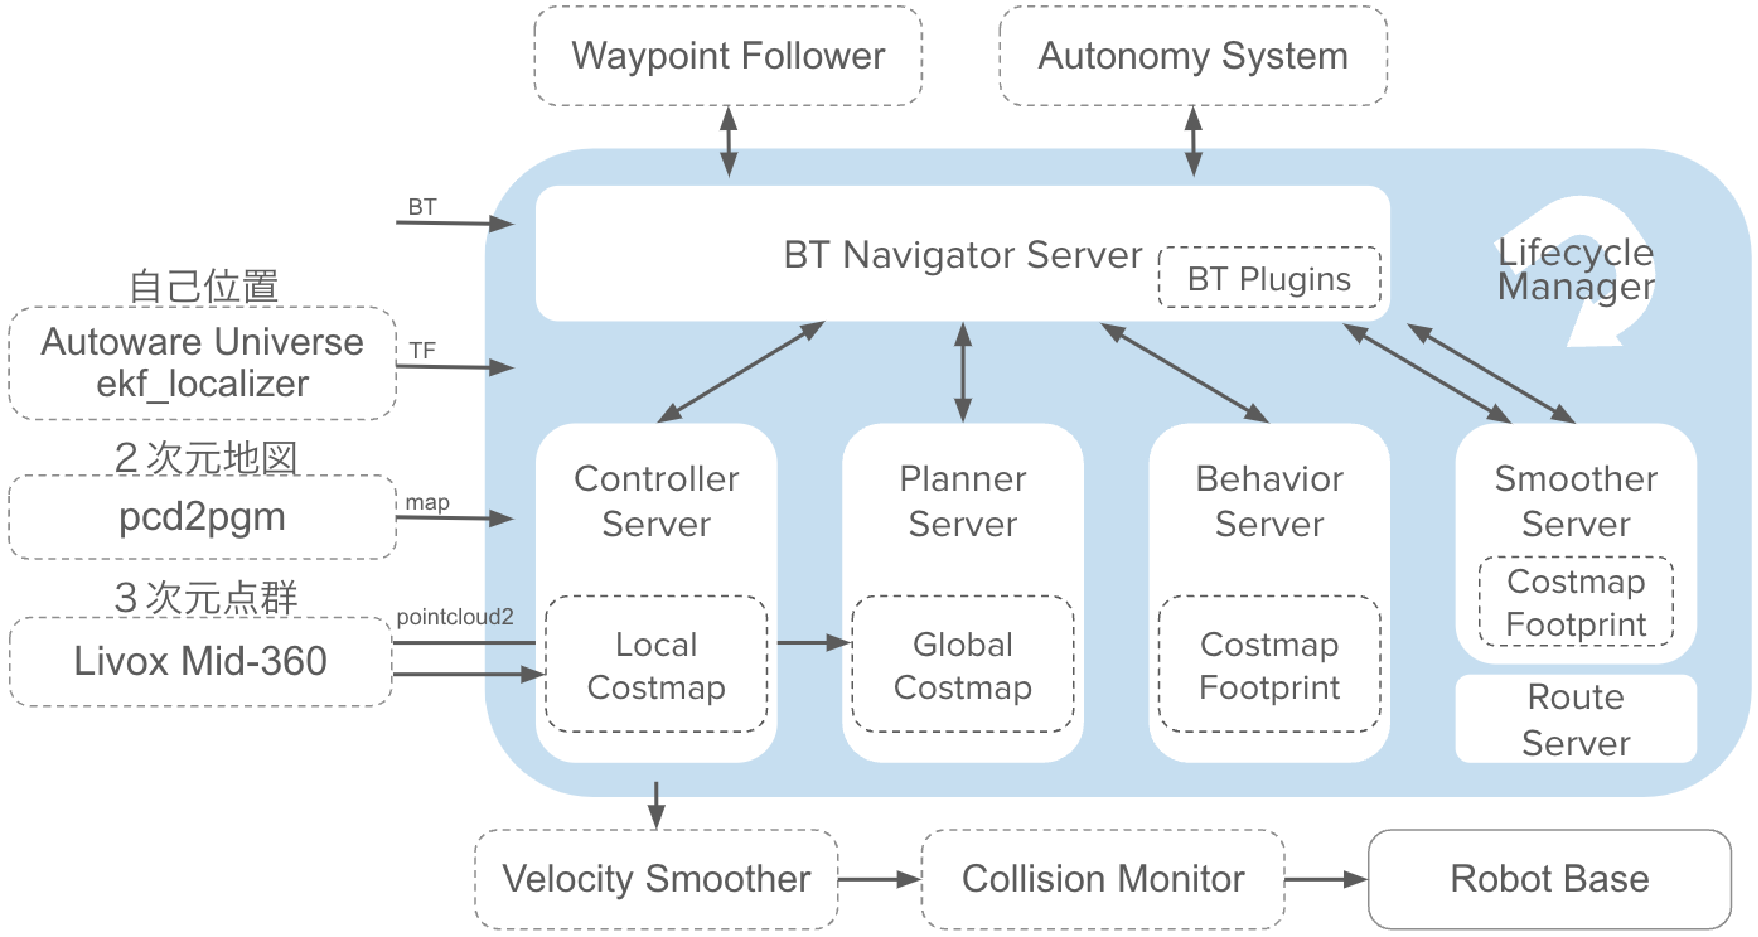
\includegraphics[width=1.0\linewidth]{figs/mugimaru_system.pdf}
    \caption{むぎまるチームのシステム構成}
    \label{fig:mugimaru_system}
  \end{center}
\end{figure}

%\begin{figure}[h]
%  \begin{center}
%      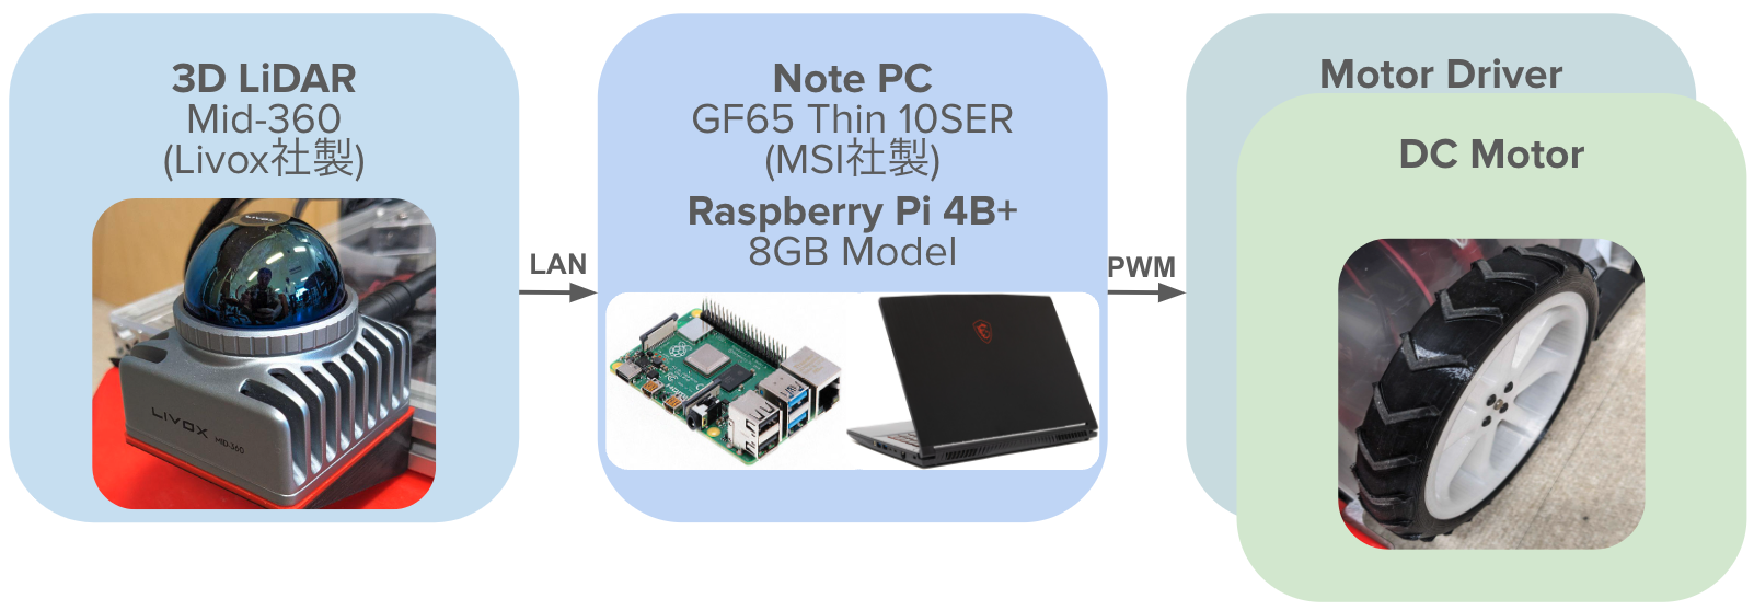
\includegraphics[width=1.0\linewidth]{figs/mugimaru_hard.pdf}
%      \caption{むぎまるチームのハードウェア構成}
%      \label{fig:mugimaru_hard}
%  \end{center}
%\end{figure}


%\section{本走行でのリタイアの原因}
\section{本走行・実験走行の結果}
\subsection{本走行の結果}

つくばチャレンジ2024での本走行の結果を表\ref{MainRun}に示す。

\begin{table}[H]
  \caption{各チームの本走行の結果}
  \label{MainRun}
  \begin{tabular}{|c|c|p{4.0cm}|}
    \hline
    走行距離 & リタイアの理由                                                                                             \\
    \hline
    429[m]   & 目標である確認走行区間完走を達成したため                                                           \\
    \hline
  \end{tabular}
\end{table}

%@@@ここの2段落、中途半端なので3.1以降に入れるか、しっかり概要を説明する@@@
%ツナチームは確認走行区間を走りきったが、最後の障害物回避の課題で、
%障害物を回避できず衝突し、失敗した。

%たまチームについては、表の通り、
%坂道において車輪を取られてしまい失敗した。
%坂道周辺では植え込みを用いて自己位置推定を試みたが失敗してしまった。

本走行の結果は表の通り、確認走行区間を完走して終了を申告したため、
429[m]という結果になった。
確認走行区間より先の区間については今年度のメインターゲットではなく、
自己位置推定に使用する地図の作成が完了していなかったため、本走行を行わなかった。

\subsection{本走行・実験走行で見つかった課題}

本チームは、10/6、10/26、10/27、11/9、11/10、11/25、12/6、12/7、12/8の計9日間、実験走行および本走行に参加した。
これらの走行で見つかった課題を以下に上げる。
\subsubsection{地図と実際の環境との違い}
実験走行において、スタート地点付近のテントの設置場所によっては、
市役所の壁が遮られ自己位置をロストしてしまうという課題があった。
この課題は、〜と考えたため、点群の更新頻度を下げることで解消した。

\subsubsection{グローバルプランナーの経路選択}
本チームが使用したグローバルプランナーは、地図上にある障害物や侵入可能領域外との境界からできるだけ離れたルートを選択する。
これにより、市役所裏側の道路では障害物が少ないため、道路の中心を走行してしまうという課題があった。
この課題は地図上の進入可能領域を狭くし、道路の端しか通ることができないようにすることで解消したが、
進入可能領域を狭くすることは自己位置ロストのしやすさとトレードオフの関係にある。
そのため、今後はグローバルプランナーの調整により障害物からできるだけ離れるような
経路選択を行わせないようにすべきであると考えられる。

\subsubsection{旋回によるオドメトリーのずれ}
確認走行区間を超えた先の地図づくりを行う中で、回転方向のオドメトリーがずれてしまうという課題があった。
この課題は現時点では解消することができていないが、ヨー方向のずれが大きいことから
IMUの情報を組み合わせて推定することにより解消できると考えられる。

\subsubsection{3次元点群の抽出高さ}
実験走行の中で、車止めを検知することができず衝突してしまうという課題があった。
これは3次元点群を2次元に切り出す高さのパラメータチューニングにより解消したが、
3次元点群を2次元に切り出す高さを低くすることは、地面勾配へのロバスト性とトレードオフの関係にある。
そのため、今後これらのトレードオフを解消できるような地面と障害物を区別するようなロジックが必要であると考えられる。


%\paragraph{障害物回避の不安定さ}
%本走行時、ike\_navの障害物回避の機能にはバグが含まれていた。
%A*によって障害物回避をするようなパスを生成し、それを追従することで障害物回避としていた。
%このA*では、推定位置からゴールまでの最短経路を導出しつつ、障害物回避を行うために、
%独自のヒューリスティック関数を実装した。
%これが、うまく実装できていれば良かったが、距離が遠いほど障害物回避を回避しようとしなくなるような
%実装となっていた。そのため今後は,障害物回避の安定のために,このヒューリスティック関数の実装を見直し,修正をする予定である.

% \paragraph{尤度場、コストマップの作成に時間がかかる}
% ike\_navでは、尤度場とコストマップを自律走行を開始させる前に作成する処理がある。
% 地図としては、確認走行区間のみの情報しかないが、
% この処理に、1分ほどかかってしまっていた。
% これは、尤度場、コストマップの作成の実装に問題があるため、
% 作成部分の実装を見直し、修正をする予定である。
% @@@1分くらいいいんじゃない?@@@

%\subsection{たまチーム}
%\subsubsection{本走行・実験走行で見つかった課題}
%\paragraph{ロボットの旋回による自己位置の破綻}


%たまチームはつくばチャレンジEXでの屋内での自律走行を実施した。
%その際、IMUを搭載していなかったため、
%ナビゲーション中にロボットが人混みを避けようとして頻繁に旋回し、
%自己位置が破綻するという課題が生じた。
%この課題への対策としてIMUを実装し、
%速度指令値から求めた角速度を積分した値であるヨー軸の角度を、
%IMUから得られるヨー方向の角速度の積分値に置き換えた。
%その結果、
%ナビゲーション中には何度も障害物を回避しようとして旋回することがあったが、
%これらの旋回が自己位置推定の破綻には繋がらなかったという結果が得られた。


%IMUの搭載による効果は、
%マッピングの際にも確認できた。
%マップの取得では、
%人がコントローラを用いてロボットを操作した。
%IMUを搭載していなかった際には、
%操作ミスやタイヤのスリップによる不要な旋回が原因で、
%歪んだマップが生成されることがあった。
%しかし、IMUの搭載によりマップの歪みが減少した。
% マップの比較画像 %


%\paragraph{マップの歪みが解消しきれていない課題}


%IMUを搭載してマッピングを行ったが、
%ループクローズが行われず、
%結局歪んだマップしか取れなかった。
%この問題に対処するため、
%最終的にペイントツールを使用して人力で歪みを修正した。
%しかし、これは根本的な解決ではなく、
%問題の原因を究明し、
%本質的な解決策を見つける必要がある。

%\subsection{むぎまるチーム}
%\subsubsection{本走行・実験走行で見つかった課題}

%むぎまるチームの本走行・実験走行で見つかった課題は,障害物回避の失敗,3次元地図と2次元地図のズレ,消費電力の大きさである.
%障害物回避の失敗については表1のとおりである.
%本チームでは自己位置推定に使用する地図には,3次元点群地図を使用し,ナビゲーションには2次元の占有格子地図を使用している.
%2次元の占有格子地図は3次元地図を基に生成しているが,
%3次元上の障害物を2次元上に投影する際,坂のある地形ではズレが生じる.
%3次元点群地図では,ロール方向のズレと,ピッチ方向のズレが存在するため,必然的に2次元平面上に投影すると誤差が生じる.
%本チームは、あまり坂道の存在しない環境でロボットの動作確認をしていたため,
%つくばチャレンジでの環境では想定以上の差が生じてしまった.

%消費電力については,むぎまるチームでは
%ノートPCの消費電力が当研究室の他チームに比べて大きくなった。
%3次元点群ベースの自己位置推定を行う負荷がその原因となった。
%2次元より3次元のセンサ処理の
%負荷が大きくなることは仕方ないかもしれないが、
%処理の軽量化も課題としたい。

\section{その他の試み}
本章では、自律走行時において未実施である、
選択課題B信号認識横断についての取り組みの取り組みついて紹介する。
\\ 本年度は確認走行区間の達成であったが、今後選択課題に挑戦することを見据えて信号認識横断の課題を取り組んだ。
本課題を選択した理由は、ロボットの機体がその場になくてもデータ収集と手法確認を行え、個別に開発を進められるためである。
本課題では、日の当たり方が大きく異なる信号をミスなくかつ素早く検出することが求められる。
そのためカメラはホワイトバランス調整などが行えるものであり、
加えて、チームの目的も踏まえると安価であることが好ましい。
そこでカメラにはスマートフォンを採用した。
一般的なスマートフォンには上記の機能が備わっており、旧型モデルを用いることで価格も抑制できる。
本チームでは2020年発売のGalaxy A21 SCV49を採用した。
\\ 本課題を達成するには、歩行者用信号(以下、信号)の検出の他に横断歩道内で停止している自動車の有無の確認などの安全確認が求められる。
この問題に対して深層学習による物体認識を用いることで対処する。
物体認識に用いる学習済みモデルは、VIDVIP\cite{BabaVIDVIP}が提供している,vidvipo\_yolov8nとした。
このモデルは、交通認識に特化したものであり、歩行者信号の赤青それぞれラベル付けされているため追加学習の必要がなく、かつYOLOv8であるため認識が比較的高速である。
\\ 
このモデルに対して、事前に取得した課題コース上から撮影した動画を認識させたところ、青信号が検出できない場合が存在することを確認した。
そこで、赤信号はYOLOによって発見し、赤信号から青信号への切り替わりは、信号の上部分の赤領域と、下部分の青部分の明度を比較することで対処した。
\\ 今年度は、信号の動画取得と、GPUを搭載したノートパソコン上で動作確認を行った。
来年度では実機への搭載を目指し、ゴールまでに十分な確保や手法の簡略化、多様な環境での安定認識などの課題に対して取り組む予定である。
また、スマートフォンのディスプレイを活用し、ロボットの状態表示や一時停止の解除機能も合わせて開発を行いたい。

\section{結言}
センサとしてLiDAR,IMUを搭載した小型ロボットでつくばチャレンジに参加した.
今回はROSのサポート終了に伴い,
ROS 2に移行したソフトウェア構成で参加した。それに加え、
IMUや3次元LiDARの追加,自作のナビゲーションスタックの使用など,
例年とは異なる試みをした。
来年度は今年度の開発内容をもとに,見つかった課題への対策や,
今回開発が間に合わなかった機能の追加をし,
小型ロボットでのコースの完走を目指す.


\section*{謝辞}
つくばチャレンジ実行委員会,つくば市の皆様に感謝申し上げます.
上田研究室の新井亮大氏、登内リオン氏,松井大和氏,山崎政光氏,林原研究室の皆様には,つくばチャレンジ 2023の参加にあたりご意見,ご協力頂き感謝申し上げます.
%↑上田整理。あと、著者に名前を連ねない人がいたらここに書くと良いです。

% 参考文献
% \small
\footnotesize
\begin{thebibliography}{99}

  \bibitem{ROS 2}
  Macenski, Steven {\it et al.}: ``Robot Operating System 2: Design, architecture, and uses in the wild,''
  Science Robotics, Vol. 7、No. 66, 2022.

  \bibitem{emcl2}
  Ryuichi Ueda: ``ryuichiueda/emcl2,'' \url{https://github.com/ryuichiueda/emcl2} (last visit: 2024-01-01).

  \bibitem{emcl2_ros2}
  Ryuichi Ueda: ``CIT-Autonomous-Robot-Lab/emcl2\_ros2,'' \url{https://github.com/CIT-Autonomous-Robot-Lab/emcl2_ros2} (last visit: 2024-01-01).


  \bibitem{RTshop}
  株式会社アールティ: ``Raspberry Pi Cat 屋外でも動かせる中型2輪ロボット'',
  RT Robot Shop Products,\url{https://rt-net.jp/products/raspberry-pi-cat/} (last visit 2024-01-05)

  \bibitem{池邉2022}
  池邉 龍宏,内田 璃空,畑中 優一郎,臼井 温希,庄司 史門,松井 大和,山崎 政光,登内 リオン,林原 靖男,上田 隆一: Raspberry Pi のみを計算に用いる小型移動ロボットでのつくばチャレンジ 2022 参加レポート,つくばチャレンジ2022シンポジウム予稿集,2022.

    \bibitem{ROS}
  Morgan Quigley {\it et al.}: ``ROS: an open-source Robot Operating System,''
  Open-Source Software workshop of the International Conference on Robotics and Automation、2009.

  \bibitem{Fusion360}
  Autodesk,\url{https://www.autodesk.com/jp/products/fusion-360/overview?term=1-YEAR&tab=subscription#top} (last visit 2025-02-02)

  \bibitem{Onshape}
  PTC,\url{https://www.onshape.com/en/} (last visit 2025-02-02)

  %\bibitem{fox2003}
  %Dieter Fox:
  %``Adapting the Sample Size in Particle Filters Through KLD-Sampling,''
  %International Journal of Robotics Research、Vol. 22、No. 12、pp. 985-1003、2003.

  %\bibitem{gutmann2002}
  %Jens-Steffen Gutmann and Dieter Fox:
  %``An Experimental Comparison of Localization Methods Continued,''
  %Proc. of the IEEE/RSJ International Conference on Intelligent Robots and Systems (IROS),pp. 454-459、2002.

  % \bibitem{ueda2002tdp}
  % 	Ryuichi Ueda {\it et al.}: 
  % ``Team description of Team ARAIBO,'' 
  % Proc. of 2002 International RoboCup Symposium、2002. 

  % \bibitem{ueda2004iros}
  % Ryuichi Ueda {\it et al.}: 
  % ``Expansion Resetting for Recovery from Fatal Error in Monte Carlo Localization -- Comparison with Sensor Resetting Methods,'' Proc.of IROS,pp.2481--2486,2004.

  % \bibitem{map2gazebo}
  % Shiloh Curtis: ``shilohc/map2gazebo'',\url{https://github.com/shilohc/map2gazebo} (last visit: 2021-12-31).

  % \bibitem{move_base}
  % Eitan Marder-Eppstein: ``move\_base,'' \url{http://wiki.ros.org/move_base} (last visit: 2021-12-31).

  %\bibitem{amcl}
  %Brian Gerkey: ``amcl,'' \url{https://wiki.ros.org/amcl} (last visit: 2021-12-31).

  %\bibitem{gmapping}
  %Brian Gerkey: ``gmapping,'' \url{http://wiki.ros.org/gmapping} (last visit: 2021-12-31).

  % \bibitem{GIMP}
  % GIMP.org: ``GIMP,'' \url{https://www.gimp.org/} (last visit: 2021-12-31).



  %\bibitem{raspicat}
  %Ryuichi Ueda and Daisuke Sato: ``ja/raspicat,'' \url{https://wiki.ros.org/ja/raspicat} (last visit: 2021-12-31).

  %\bibitem{youtube}
  %BEIKE: ``つくばチャレンジ2022 実験走行 11/19 スタートからゴールまで自律移動(神の手4回),'' \url{https://www.youtube.com/watch?v=3gpjVhRIJDY} (last visit: 2022-12-12).

  % \bibitem{raspicat_rosbag}
  % Tatsuhiro Ikebe: ``uhobeike/raspicat\_rosbag,'' \url{https://github.com/uhobeike/raspicat_rosbag} (last visit: 2021-12-31).

  %\bibitem{池邉2021}
  %池邉 龍宏,曹 越,高橋 秀太,クルス ペレス アントニオ,林原 靖男,上田 隆一: 小型移動ロボットによるつくばチャレンジへの挑戦,第22回計測自動制御学会システムインテグレーション部門講演会,pp.3390-3393,2021.

  

  % \bibitem{上田2019}
  % 上田 隆一: ``詳解確率ロボティクス''、講談社、2019.

  %   \bibitem{上田2020}
  %  上田隆一,鈴木勇矢: 自己位置が不確かな状況における移動ロボットの危険回避行動の生成,第38回日本ロボット学会学術講演会予稿集,pp.RSJ2020AC2C2-02,オンライン開催,2020.

  % \bibitem{地図合成}
  % 川合隆太他: ``産業技術大学院大学における自律移動ロボット「産技大2号」の開発'',2019年度つくばチャレンジシンポジウム、pp.4-7、2020.


  % \bibitem{aws2020}
  %   CIT自律ロボット研究室: ``AWSロボットデリバリーチャレンジで本研究室メンバーが優勝,'' \url{https://lab.ueda.tech/?post=20200915_aws_challenge} (last visit 2022-01-04)

  % \bibitem{学科サイト}
  %   千葉工業大学先進工学部未来ロボティクス学科: ``AWS Robot Delivery Challenge 2021 準優勝''、\url{https://www.robotics.it-chiba.ac.jp/j/?p=838} (last visit 2022-01-04)

  % \bibitem{つくばチャレンジロボット仕様}
  % つくばチャレンジ実行委員会事務局:``つくばチャレンジ 2021 ロボット仕様条件'',
  % \url{https://tsukubachallenge.jp/2021/regulations/specs} (last visit 2021-12-31)

  % \bibitem{UST-30LX}
  % 北陽電機株式会社: ``UST-30LX'',\url{https://www.hokuyo-aut.co.jp/search/single.php?serial=195#spec} (last visit: 2021-12-31).

  % \bibitem{Turtlebot3 Burger}
  % 株式会社ロボティズ: ``Turtlebot3 Burgerの仕様'',\url{https://emanual.robotis.com/docs/en/platform/turtlebot3/features/} (last visit: 2022-1-3).

  % \bibitem{つくばチャレンジ公式記録}
  % つくばチャレンジ実行委員会事務局:``つくばチャレンジ2021の走行結果'',
  % \url{https://tsukubachallenge.jp/2021/records/final} (last visit 2021-12-31)

  % \bibitem{出野畑中}
  %   畑中 優一郎,出野 廣太郎,上田 隆一:``Raspberry Pi 3BのみでRaspberry Pi Catのナビゲーション(屋内環境編)'',CIT自律ロボット研究室,\url{https://lab.ueda.tech/?post=20211210} (last visit 2022-01-02)

  \bibitem{ike_nav}
  Tatsuhiro Ikebe: ``uhobeike/ike\_nav,'' \url{https://github.com/uhobeike/ike_nav} (last visit: 2024-01-10).

  \bibitem{ike_nav_detail}
  池邉龍宏: ``自作ナビゲーションスタックでつくばチャレンジ2023に挑戦してみた話'',
  \url{https://qiita.com/BEIKE/items/f3ff141cc25d49c01363} (last visit 2023-1-10).


  \bibitem{fox1999etal}
	  D. Fox {\it et al.}: ``Monte Carlo Localization: Efficient Position Estimation for Mobile Robots,''
  Proc. of AAAI, pp. 343-349, 1999.

  \bibitem{hart1968}
  Peter E. Hart and Nils J. Nilsson and Bertram Raphael: ``A Formal Basis for the Heuristic Determination of Minimal Cost Paths,''
  IEEE Transactions on Systems Science and Cybernetics, Vol. 4, No.2, pp. 100-107, 1968.

  %\bibitem{dijkstra1959}
  %E. W. Dijkstra : ``A Note on Two Problems in Connexion with Graphs,''
  %Numerische Mathematik, Vol. 1, pp. 269-271, 1959.

  \bibitem{alberto2006}
  Bemporad, Alberto: ``Model Predictive Control Design: New Trends and Tools,''
  Proceedings of the 45th IEEE Conference on Decision and Control, pp. 6678-6683, 2006.

  \bibitem{fastlio}
  Ericsii: ``Ericsii/FAST\_LIO (ros2 branch),'' \url{https://github.com/Ericsii/FAST_LIO.git} (last visit: 2023-11-19).

  \bibitem{autoware}
  The Autoware Foundation: ``autowarefoundation/autoware.universe,'' \url{https://github.com/autowarefoundation/autoware.universe.git} (last visit: 2023-11-19).

  \bibitem{nav2}
  ROS Planning: ``ros-planning/navigation2 (humble branch),'' \url{https://github.com/https://github.com/ros-planning/navigation2.git.git} (last visit: 2023-11-19).


  \bibitem{ike_nav_loc_youtube}
  池邉龍宏: ``自作パッケージで屋外自律移動してみた in つくばチャレンジ2023(本走行)'',
  \url{https://www.youtube.com/embed/k9yxRKOCa14?si=c7ISmE1wH5W4BhgU&amp;start=1365} (last visit 2024-01-05)

  \bibitem{上田2023}
上田隆一, 登内リオン, 池邉龍宏, 林原靖男: ``移動ロボットのための自己位置の不確かさを考慮したセンシングできない固定障害物の回避手法 ---価値反復を用いたナビゲーションにおける状態空間の局所拡張---'', 第28回ロボティクスシンポジア講演論文集, pp. 118-123, 2023.

  \bibitem{tonouchi2023}
  登内リオン, 池邉龍宏, 林原靖男, 上田隆一: ``価値反復を用いた移動ロボットによる屋外ナビゲーション,''
  日本機械学会ロボティクス・メカトロニクス講演会, 2P1-G06, 2023.

  \bibitem{ueda2023JRM}
  R. Ueda, L. Tonouchi, T. Ikebe, and Y. Hayashibara: ``Implementation of Brute-Force Value Iteration for Mobile Robot Path Planning and Obstacle Bypassing,''
  J. Robot. Mechatron., Vol.35, No.6, pp. 1489-1502, 2023.

  \bibitem{ikebeMECH}
  池邉龍宏, 林原靖男, 上田隆一: ``未知障害物によるモンテカルロ自己位置推定の破綻を防ぐための観測範囲の制限と選択'',
  日本機械学会ロボティクス・メカトロニクス講演会, 2A2-G06, 2023.
  
  \bibitem{BabaVIDVIP}
  T. Baba, “VIDVIP: Dataset for Object Detection During Sidewalk Travel,” J. Robot. Mechatron., Vol.33 No.5, pp. 1135-1143, 2021. https://doi.org/10.20965/jrm.2021.p1135
  
\end{thebibliography}
\normalsize

\clearpage

%\section{付録として、各実験走行でどんなことをやっていたかを書く?}
% 当チームは、9日間分のすべての実験走行会に参加した。
% 7月2日、7月23日は確認走行区間から信号あり横断歩道手前までの自己位置推定のテストを行った。
% 地図は昨年作ったものを使い、自己位置推定のパッケージにemcl2を使った。
% また、駅・公園エリアの地図作成のためのrosbagを取った。
% 9月17日、10月1日は駅・公園エリアの走行実験を行った。
% 走行エリアが増えたことに伴い地図の容量が増大し、4GBメモリのRaspberry Piでは処理できなかった。
% メモリの容量を増やし、地図の余白部分を削ることで駅・公園エリアが走行できるようになった。
% 10月22日、10月23日は信号あり横断歩道の横断の走行テストを行った。
% 通常の走行速度では青信号中に横断しきれなかったため、
% 信号あり横断歩道の横断中のみ走行速度を変えることで、青信号中に横断しきることができた。

\end{document}
